%! Author = mariuszindel
%! Date = 24.01.21

\section{Testing}


\subsection{Übersicht Begriffe \& Konzepte}
% die Einsatzzweck unterschiedlicher Testarten erklären (z.B. Integration, Regression, Load (Stress), Performance, Endurance Test, Chaos Testing, Security Tests, Usability Test).
% Unit-Tests von Integration-Tests und System-Tests unterscheiden.
\textbf{Unit Tests:} Getestet werden einzelne Klassen, Module
\textbf{Integrationstests:} Zusammenspiel 2 oder mehr ''Units''
\textbf{Funktionstests:} System entsprechend spezifizierte funktionale Anforderungen verhält
\textbf{Regressionstests:} Veränderungen im Code zu (unerwarteten) Änderungen im Verhalten
\textbf{Funktionale Systemtests:} Zusammenspiel aller Systemkomponenten in der Zielumgebung
\textbf{Weitere:} Load (Stress), Performance, Endurance Test (über 3h), Chaos Testing (Wartung/Ausfall), Security Tests, Usability Test

% beschreiben was in den Phasen (Setup, Exercise, Verify, Teardown) eines Test passiert.
\vspace{-8pt}
\begin{center}
    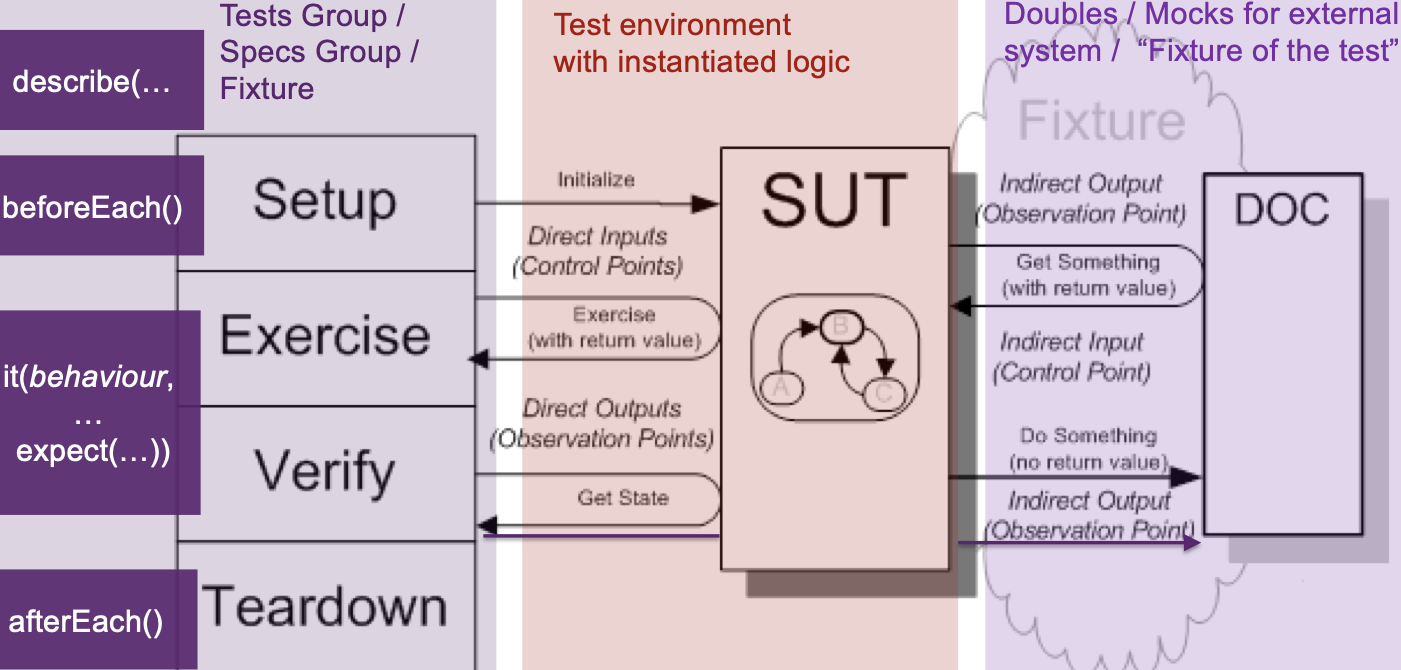
\includegraphics[width=\linewidth]{graphic/testing/Unit-Testing.png}
\end{center}
\vspace{-8pt}

\subsection{Tools}
% je zwei JavaScript Testrunner und Assertion-Libraries aufzählen.
% die Aufgaben von JavaScript Testrunner und Assertion-Libraries nennen
\begin{itemize}
    \item \textbf{Test-Runner:} Ein Rahmen der Tests entgegennimmt, ausführt und die Resultate anzeigt (Mocha, Jest)
    \item \textbf{Assertion Library:} Code zur Ausführung einzelner Tests (Chai, Assert)
\end{itemize}



\subsection{Unit Testing Patterns}
% bei gegebenem Test-Code Test-Double klassifizieren und erklären was die Aufgabe dieses Test Doubles ist.
%TODO

%das Verhalten von Test welche die vorgestellten Libraries Unit-Test und Mocking Libraries verwenden erklären.
%TODO


% einen einfachen Unit Test mit dem Mocha und Chai API schreiben.
\subsubsection{Mocha API}
\begin{lstlisting}
const assert =  require('assert');
describe( 'Array', function() {
 describe('#indexOf()', function() {
  beforeEach(function() {
   this.testArray = [1, 2, 3]; });
    it('should return -1 when the value is not present',
     function() {
      assert.strictEqual(this.testArray.indexOf(4),
       -3); /*should be -1*/ }); });});
\end{lstlisting}

\subsubsection{Chai API}
\begin{lstlisting}
const {expect} =  require('chai');
describe( 'Array', function() {
 describe('#indexOf()', function() {
  beforeEach(function() {
   this.testArray = [1, 2, 3]; });
    it('should return -1 when the value is not present',
     function() {
      expect(this.testArray.indexOf(4)).to.equal(-3);
       });});});
\end{lstlisting}


\subsection{Unit Test Smells}
% Test-Smells erkennen und Refactorings zur Verbesserung der Tests durchführen.
Probleme: Tests die...
\begin{itemize}
    \item ... zu viele expect enthalten
    \item ... nicht alle If/else prüen
    \item ... schwierig zu verstehen sind
    \item ... zu lange dauern
    \item ... sich wiederholen
    \item ... if Logik verwenden
\end{itemize}

\vfill
$ $

\columnbreak
